%%%%%%%%%%%%%%%%%%%%%%%%%%%%%%%%%%%%%%%%%%%%%%%%%%%%%%%%%%%%%%%%%%%%%%%%
% Plantilla TFG/TFM
% Universidad de A Coruña. Facultad de Informática
% Realizado por: Welton Vieira dos Santos
% Modificado: Welton Vieira dos Santos
% Contacto: welton.dossantos@udc.es
%%%%%%%%%%%%%%%%%%%%%%%%%%%%%%%%%%%%%%%%%%%%%%%%%%%%%%%%%%%%%%%%%%%%%%%%


\chapter{Desarrollo técnico}
\section{Videojuego en 2D}
\subsection{Descripción}ISS Manticore es un scroll lateral con ligeros tintes de metroidvania\footnote{Metroidvania: es un subgénero de juego basado en un concepto de plataformas no lineal con un mundo conectado que fomenta que el jugador lo explore} en el diseño de escenarios al tener algunos incentivos para desviarse del camino principal, pero dividido en niveles donde los jugadores comienzan cada fase en el extremo izquierdo de un escenario lineal.

Su objetivo es alcanzar la salida de la nave de la cual se ha quedado atrapado en el momento que ha intentado entregar un paquete en la misma.

El protagonista va avanzando y derrotando los enemigos que contiene en cada fase.
\subsection{Personajes}
Jackie, el protagonista del juego tendrá que completar distintas fases, en las que tendrá que superar distintos enemigos y acometer distintas tareas para alcanzar su objetivo, para ello el jugador tendrá que mover al protagonista empleando las flechas del teclado para avanzar, esquivar a los enemigos y recoger los coleccionables necesarios y disparando con un click de ratón a los distintos personajes que se interpongan en su camino.

\subsection{Enemigos}
Los enemigos se interponen en el camino del protagonista habitando los diferentes escenarios por los que avanza dañando al protagonista si este entra en contacto con los enemigos. 
\begin{itemize}
    \item \textbf{Octopus:} Estos pequeños seres extraños se encuentran levitando en una misma posición con el objetivo de interrumpir al protagonista en su camino para completar su cometido. Ejemplo en la Figura \ref{fig:Octopus}.
    \item \textbf{Tortugas:} Están en constante movimiento de un lado a otro y dificultan el transcurso del personaje, que debe abatirlos o esquivarlos, para no salir dañado y conseguir completar su misión. Ejemplo en la Figura \ref{fig:Tortuga}.
    \item \textbf{Spiderbots:} Son el enemigo más difícil de derrotar para el protagonista debido a que dispara proyectiles cada 10 segundos que pueden dañarlo si no es capaz de esquivarlos. Ejemplo en la Figura \ref{fig:Octopus}. 
\end{itemize}

\subsection{Diseño}
\subsubsection{Patrón estrategia}
Este patrón ha sido utilizado en la gran mayoría del código, con la idea de abstraer en clases una serie de estados y comportamientos y, a medida que se se van extendiendo otras clases de una forma bastante jerárquica, haciendo que el comportamiento sea cada vez más específico, por ejemplo el Menu principal del juego que está compuesto por varios componentes como imágenes, botones (estilo rolover) para seleccionar las opciones pertinentes.

\subsubsection{Patrón Singleton}
El patrón singleton está presente en la clase Director, GestorRecursos y tambien en las factorías de los personajes y de las fases del juego. Además de solamente permitir que se instancia solamente un objecto con el uso de clases internas en el caso del director, que solamente tiene uno en todo el proceso.

\subsubsection{Personajes}
La implementación de los personajes hereda de la clase MiSprite y va jerarquizando como se muestra en la Figura \ref{fig:Personaje}. Esa clase incorpora los elementos necesarios para almacenar las posiciones, sprites, velocidades y todos los elementos comunes como el scroll.

\begin{figure}[H]
	\centering
	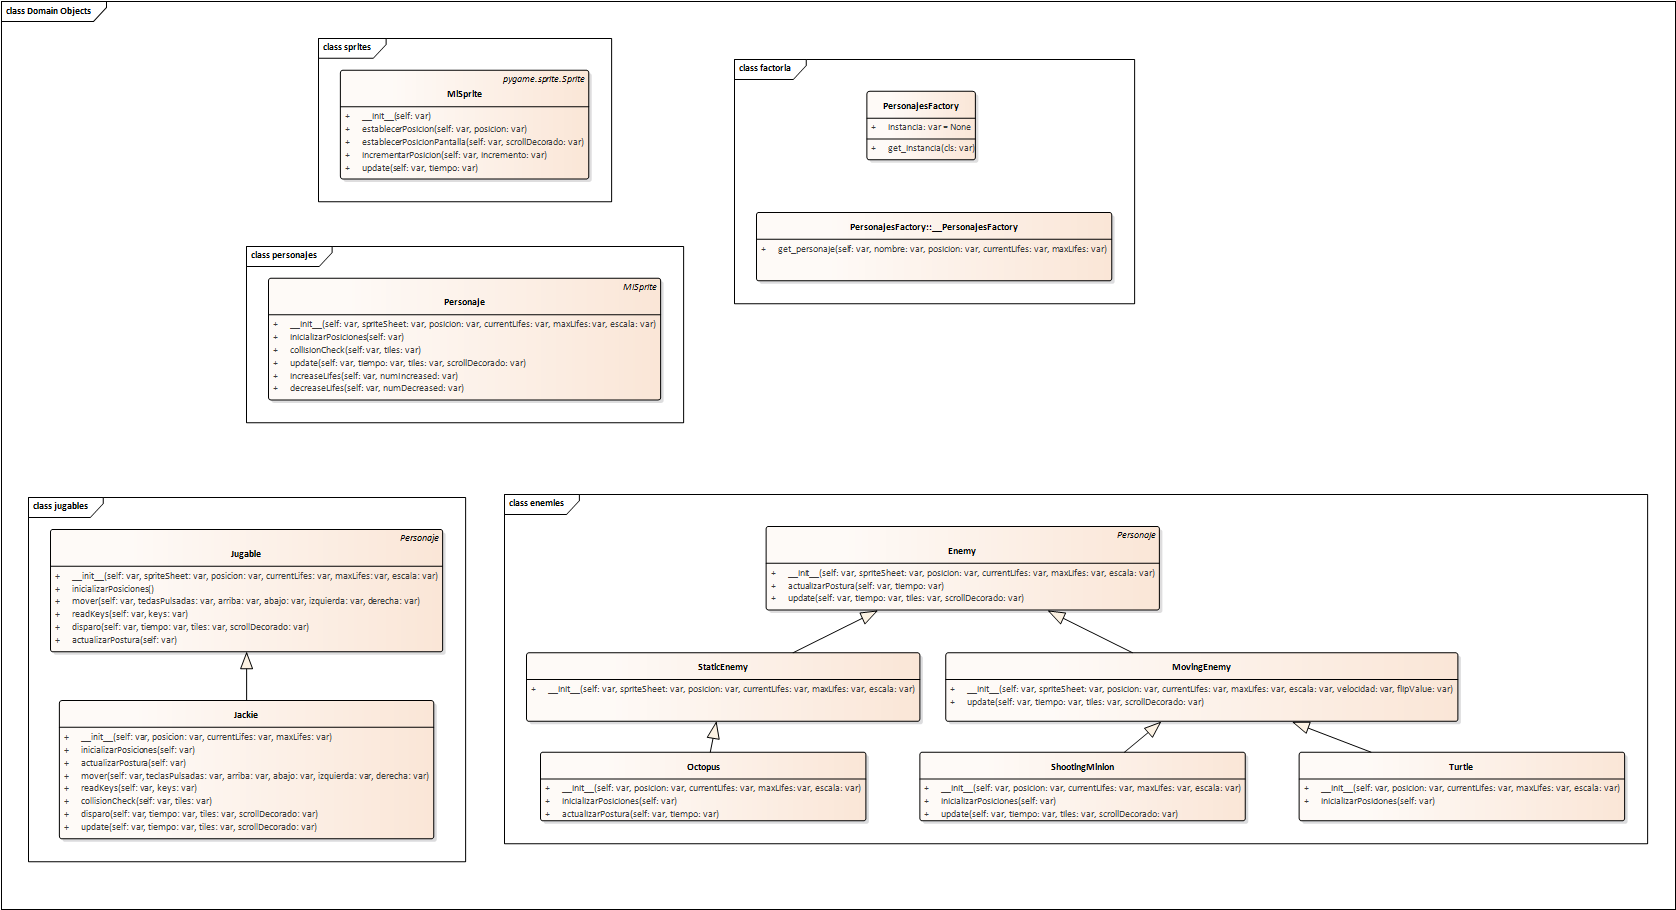
\includegraphics[scale=0.30]{imagenes/Personaje.png}
	\caption{\label{fig:Personaje}Ejemplo de la jerarquía de la clase Personaje}
\end{figure}

Cada objeto del tipo personaje es instanciado por su factoría correspondiente con la intención de permitir un mejor mantenimiento y expansión del código futuramente.

Esos personajes están diferenciados por dos tipos básicos, uno jugable y otro los enemigos.

\subsubsection{Fases}
La implementación de la dinámica de fases es muy similar a la dinámica de los personajes como se puede apreciar en la Figura \ref{fig:Fases} concervando los métodos ``update'', ``eventos'' y ``dibujar'' de la clase Escena.

\begin{figure}[H]
	\centering
	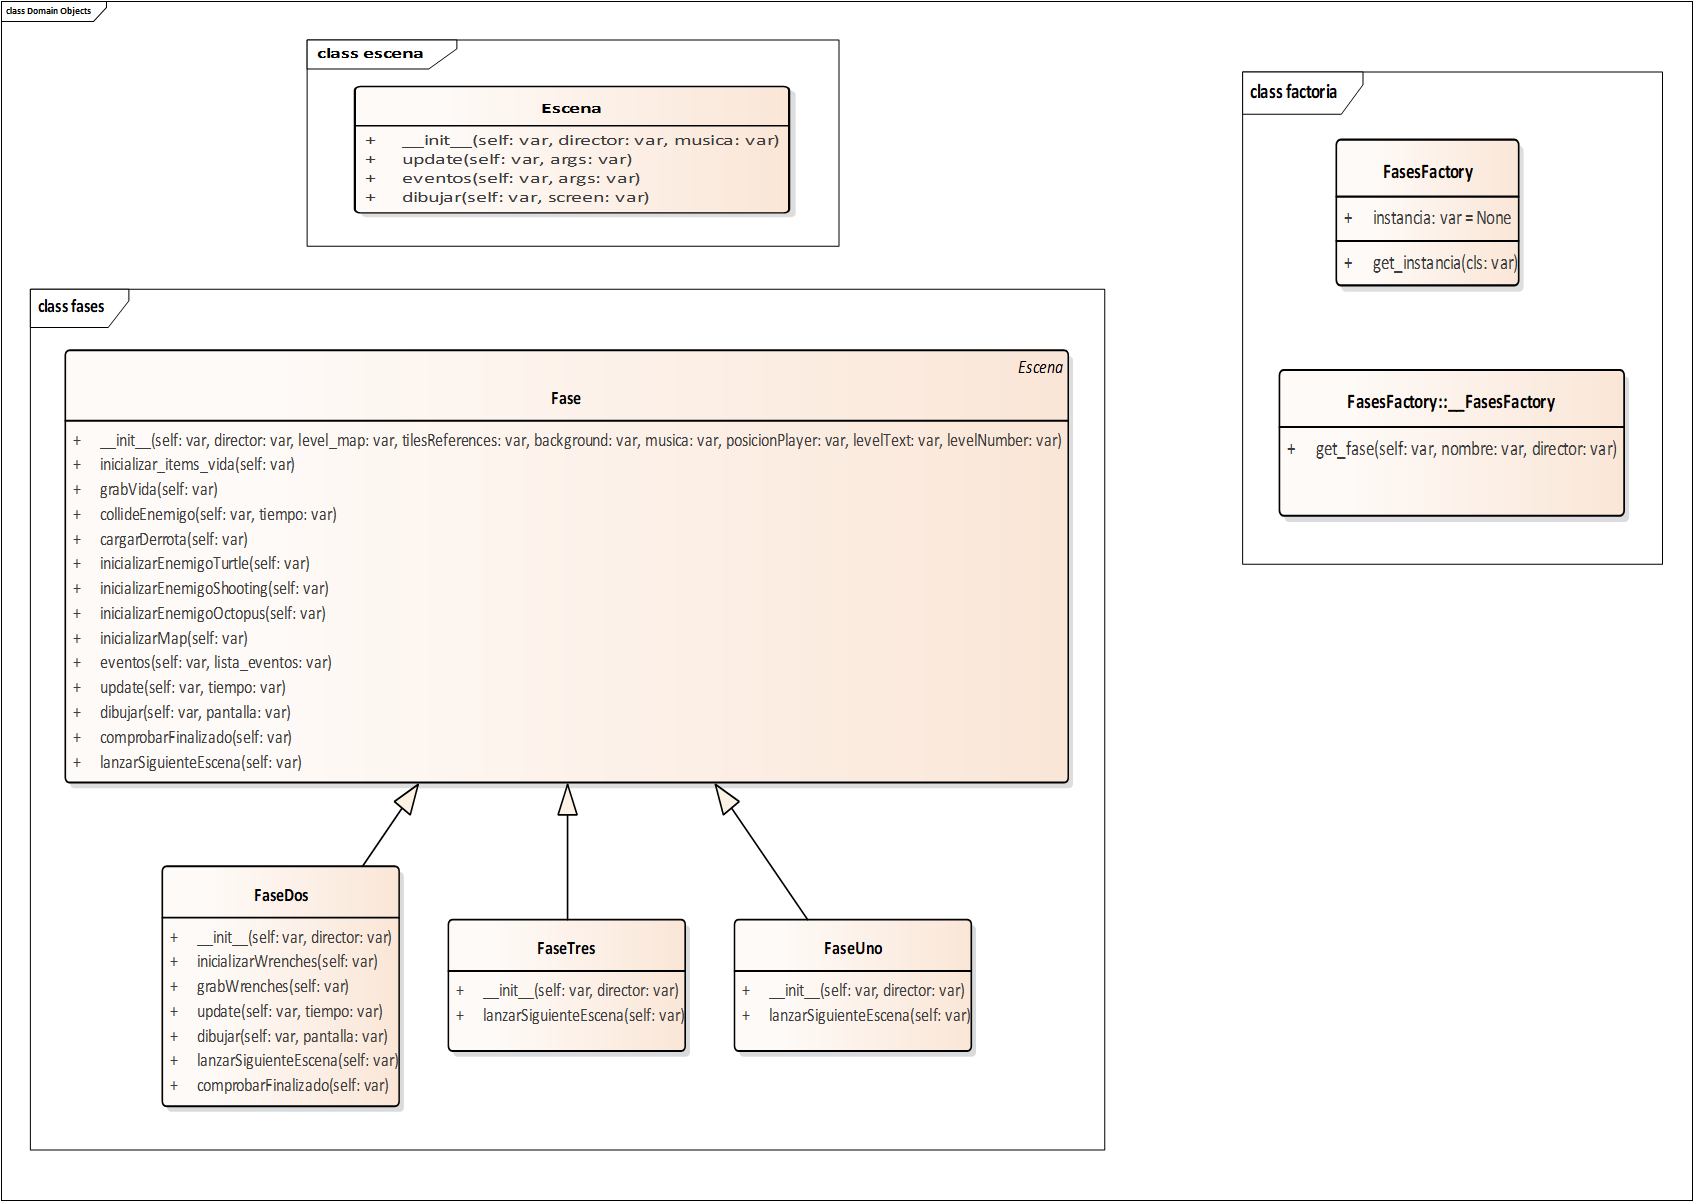
\includegraphics[scale=0.30]{imagenes/Fases.png}
	\caption{\label{fig:Fases}Ejemplo de la jerarquía de la clase Fase}
\end{figure}

\subsubsection{Escena}
La clase Escena define toda las estructura visual del juego, donde desde ahí se puede controlar los menus, personajes, transiciones y etc.

La clase Escena posee tres métodos principales:
\begin{itemize}
	\item eventos: Encargado de leer los eventos producidos por la interacción del usuario con el sistema.
	\item update: Encargado de actualizar el modelo de escena en cuestión basado en los eventos producidos durante la interacción del usuario.
	\item dibujar: Encargado de dibujar los elementos de la parte visual del juego.
\end{itemize}

\subsubsection{Director}
El director es el encargado de ejecutar la escena pertinente, que puede ser un menú o las fases correspondientes de las determinadas etapas del juego. La Figura \ref{fig:Director} muestra su estructura.

\begin{figure}[H]
	\centering
	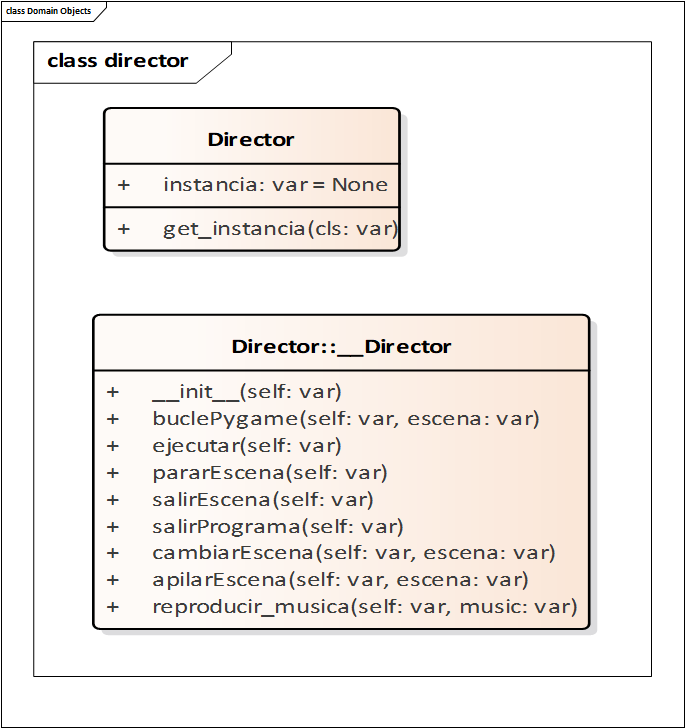
\includegraphics[scale=0.30]{imagenes/Director.png}
	\caption{\label{fig:Director}Ejemplo de la jerarquía de la clase Director}
\end{figure}

Como se puede observar, director possee una clase interna.

\subsubsection{Gestor de recursos}
Como su propio nombre dice, es el encargado de suministrar los recursos necesarios para la una buena interacción con el juego. La Figura \ref{fig:GestorRecursos}

\begin{figure}[H]
	\centering
	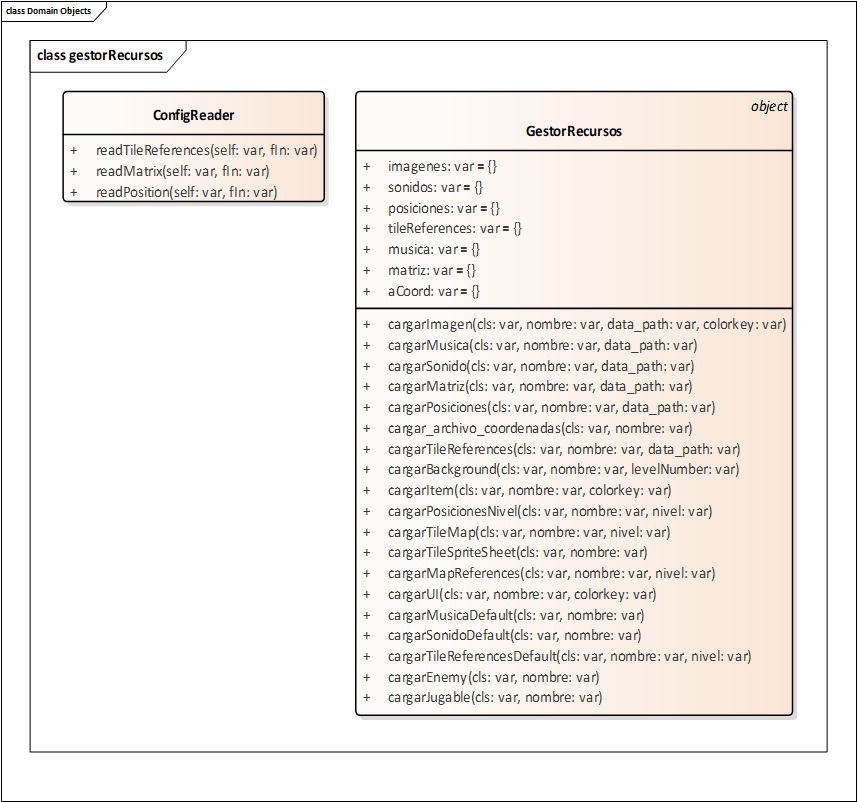
\includegraphics[scale=0.30]{imagenes/GestorRecursos.png}
	\caption{\label{fig:GestorRecursos}Ejemplo uml del gerenciador de recursos}
\end{figure}

\subsection{Escenas}

La transición entre escenas se muestra en el diagrama de la Figura \ref{fig:TrasicionEscenas}. 

\begin{figure}[H]
	\centering
	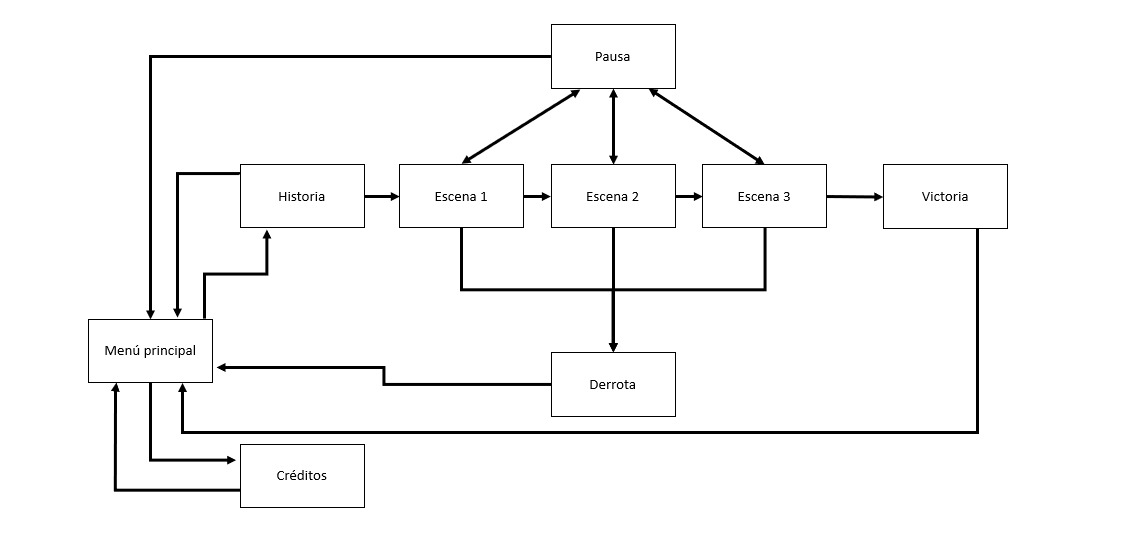
\includegraphics[scale=0.35]{imagenes/transicionEscenas.jpeg}
	\caption{\label{fig:TrasicionEscenas}Diagrama de transición de las escenas}
\end{figure}

\subsubsection{Menú principal}
En esta primera pantalla (Figura \ref{fig:EjemploMenuPrincipal}), que se muestra al jugador nada más ejecutar el juego, se le permite elegir entre comenzar con la historia, visualizar los créditos, lo que enviaría al usuario a la pantalla de Créditos, o la opción de salir, que cerraría el juego. 

\begin{figure}[H]
	\centering
	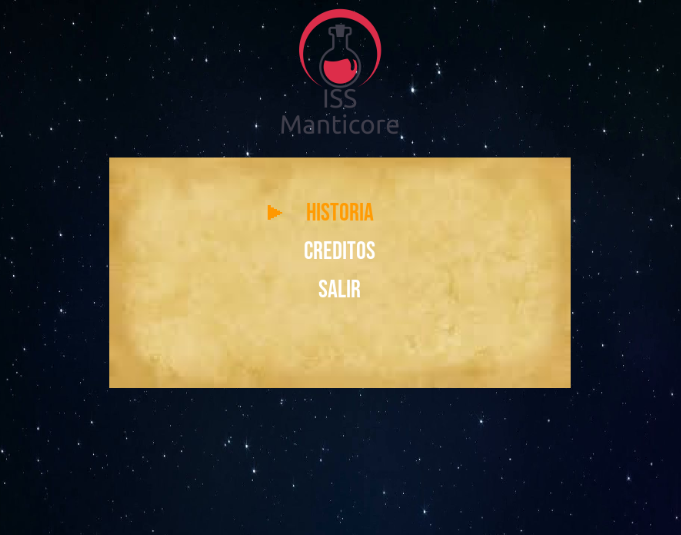
\includegraphics[scale=0.50]{imagenes/EjemploMenuPrincipal.png}
	\caption{\label{fig:EjemploMenuPrincipal}Ejemplo del menu principal}
\end{figure}

\subsubsection{Historia}
Esta pantalla (Figura \ref{fig:EjemploMenuHistoria})muestra un breve resumen de la historia y la leyenda del juego, en la que se puede ver la configuración inicial que contiene la imagen del personaje, el número de vidas inicial, el número de proyectiles con el que cuenta antes de comenzar la aventura (con miras a añadir más adelante objetos de munición y diferentes armas o proyectiles). Desde esta pantalla se puede volver al Menú principal pulsando la tecla Esc o pasar a la Escena 1 pulsando la tecla Enter. 

\begin{figure}[H]
	\centering
	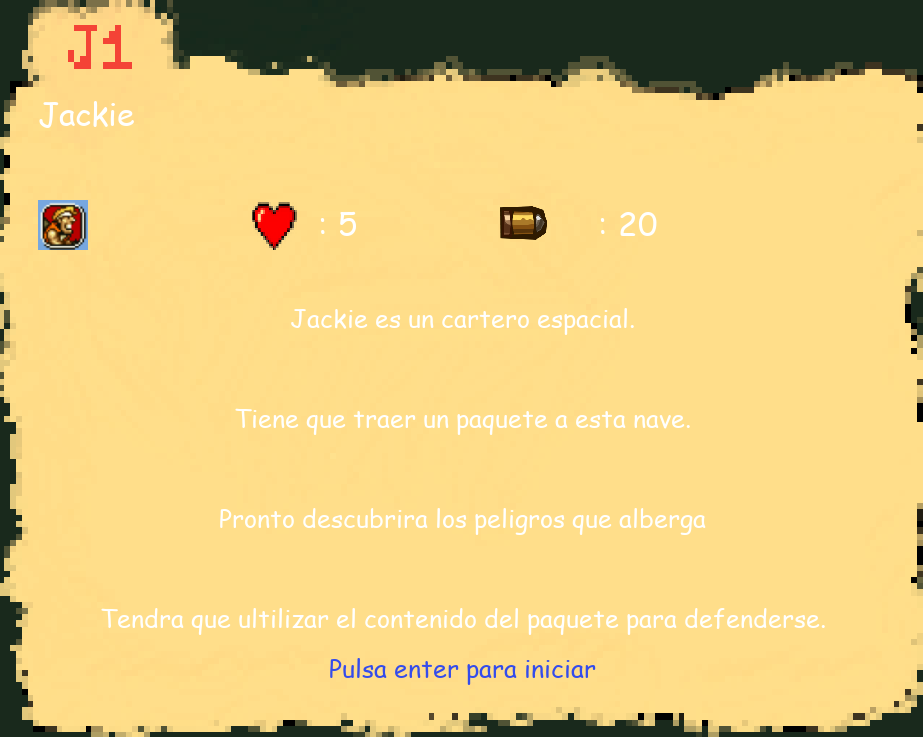
\includegraphics[scale=0.50]{imagenes/EjemploMenuHistoria.png}
	\caption{\label{fig:EjemploMenuHistoria}Ejemplo del apartado historia del menu principal}
\end{figure}

\subsubsection{Fase 1 - Sala de calderas}
La escena comienza con el protagonista en la sala de calderas, este emprende su aventura con tres vidas, que podrá aumentar o disminuir segundo se desenvuelva, nada más arrancar aparece el primer enemigo, un spiderbot al que tendremos que derrotar, si seguimos avanzando nos encontramos con el segundo enemigo, en este caso un octopus, y también con el primer botiquín, que nos permitirá ganar una vida, continuando con la aventura nos encontraremos con más enemigos a los que tendremos que derrotar, para llegar al final de esta escena. 

Para pasar a la siguiente escena deberemos continuar andando al llegar al final del escenario.  

En ese nivel nuestro personaje encontrará con distintos enemigos que una vez superados se terminará esa fase del del juego. La Figura \ref{fig:EjemploEscena_1} muestra un ejemplo de la escena 1. 

\begin{figure}[H]
	\centering
	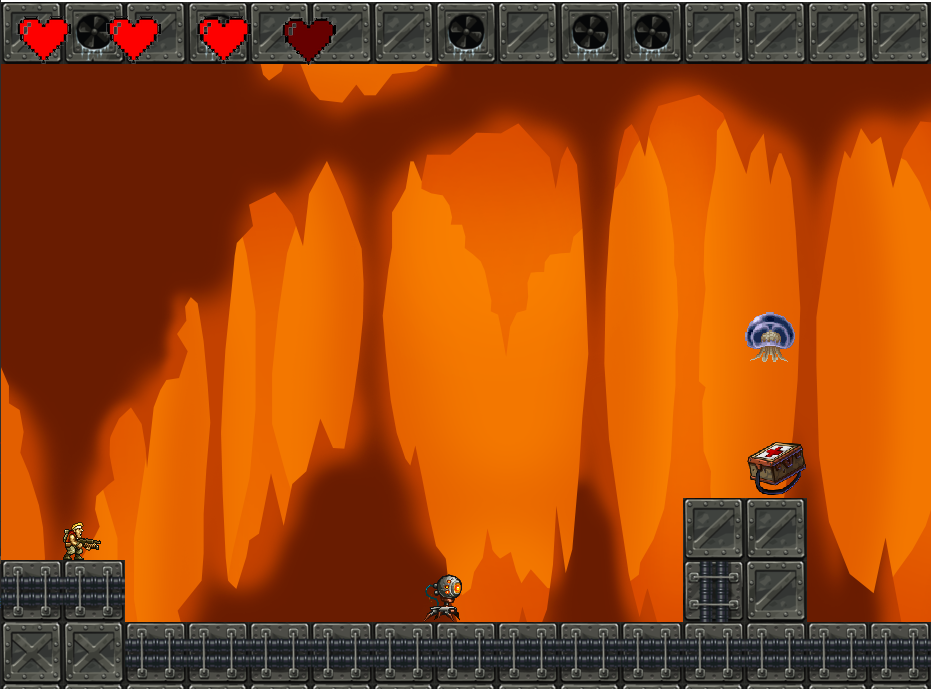
\includegraphics[scale=0.50]{imagenes/EjemploEscena_1.png}
	\caption{\label{fig:EjemploEscena_1}Ejemplo de la fase 1}
\end{figure}

\subsubsection{Fase 2 - Almacen}
En esta segunda escena el protagonista se encuentra con 3 vidas en el almacén, donde tendrá que recoger todas las herramientas (un total de 11) que se va a ir encontrando para completar con éxito esta etapa, también se encontrará con botiquines que le permitirán recuperar vidas, las cuales le podrán ser arrebatadas por los enemigos que entorpecerán su camino, tendrá que hacer frente a 7 tortugas, 6 spiderbots y 7 octopus. Si continúa andando al llegar al final del escenario, pasará a la escena 3. En la Figura \ref{fig:EjemploEscena_2} presenta un ejemplo de la misma. 

\begin{figure}[H]
    \centering
    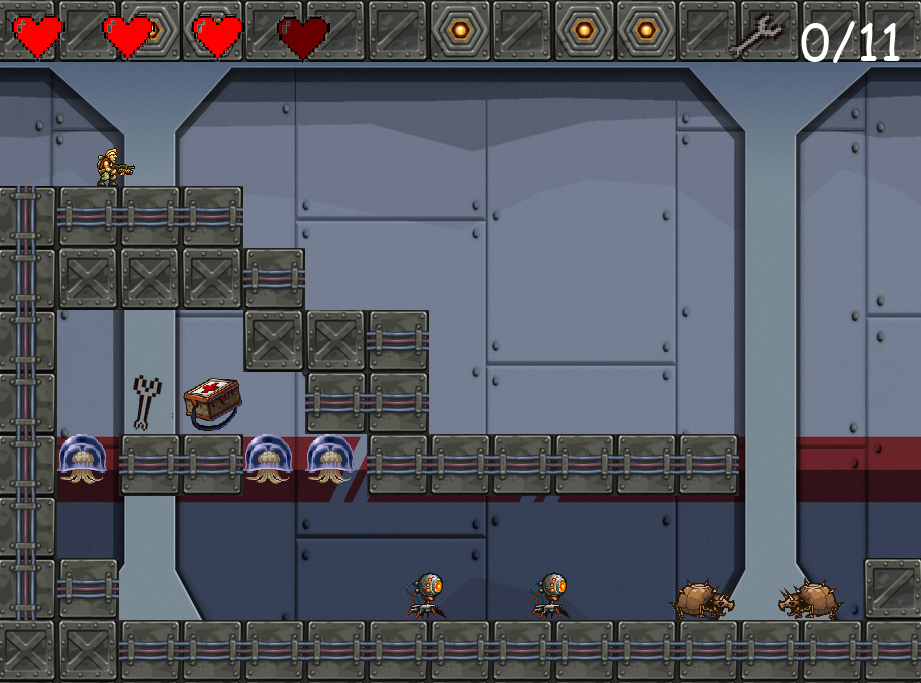
\includegraphics[scale=0.50]{imagenes/EjemploEscena_2.png}
    \caption{\label{fig:EjemploEscena_2}Ejemplo de la fase 2}
\end{figure}
\subsubsection{Fase 3 - Puente de mando de la nave}

En la tercera y última escena el jugador aparece en el Puente de mando con 3 vidas, al igual que en las escenas anteriores, debe llegar al final del escenario con vida intentando destruir a los enemigos que se encuentre a su paso, un total de 20: 7 tortugas, 7 octopus y 6 spiderbots. Si consigue llegar con vida al final de esta escena habrá completado la aventura y llegará a la pantalla de Victoria. En la Figura \ref{fig:EjemploEscena_3} presenta un ejemplo de la misma.

\begin{figure}[H]
    \centering
    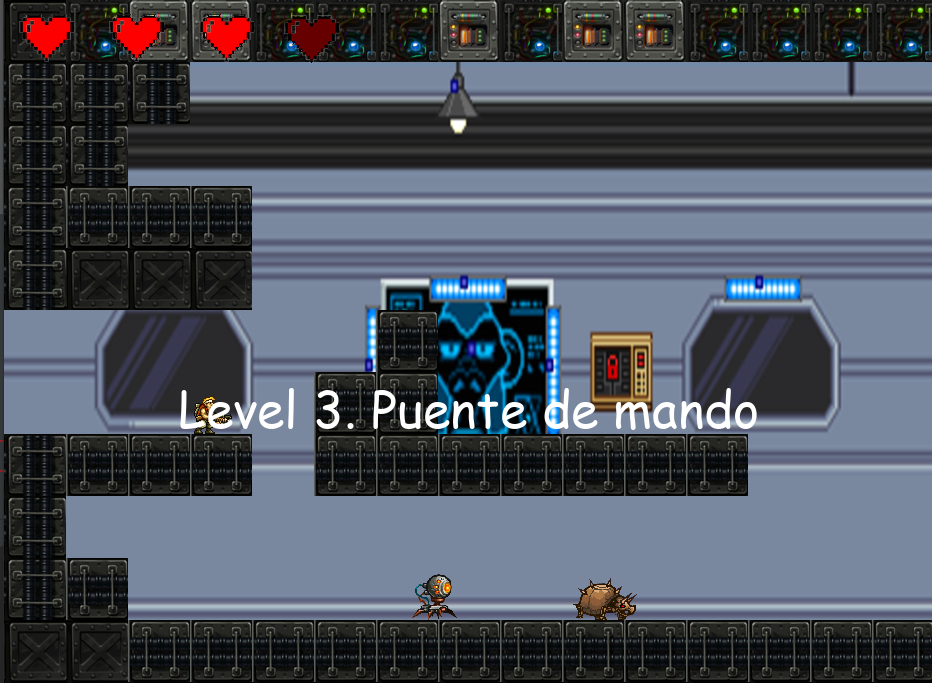
\includegraphics[scale=0.50]{imagenes/EjemploEscena_3.png}
    \caption{\label{fig:EjemploEscena_3}Ejemplo de la fase 3}
\end{figure}

\subsubsection{Créditos}
Pantalla en la que se visualiza la lista de nombres de los desarrolladores y del product owner. Desde esta pantalla se permite al jugador volver al menú principal pulsando la tecla Esc. Ejemplo en la Figura \ref{fig:EjemploCreditos}.

\begin{figure}[H]
	\centering
	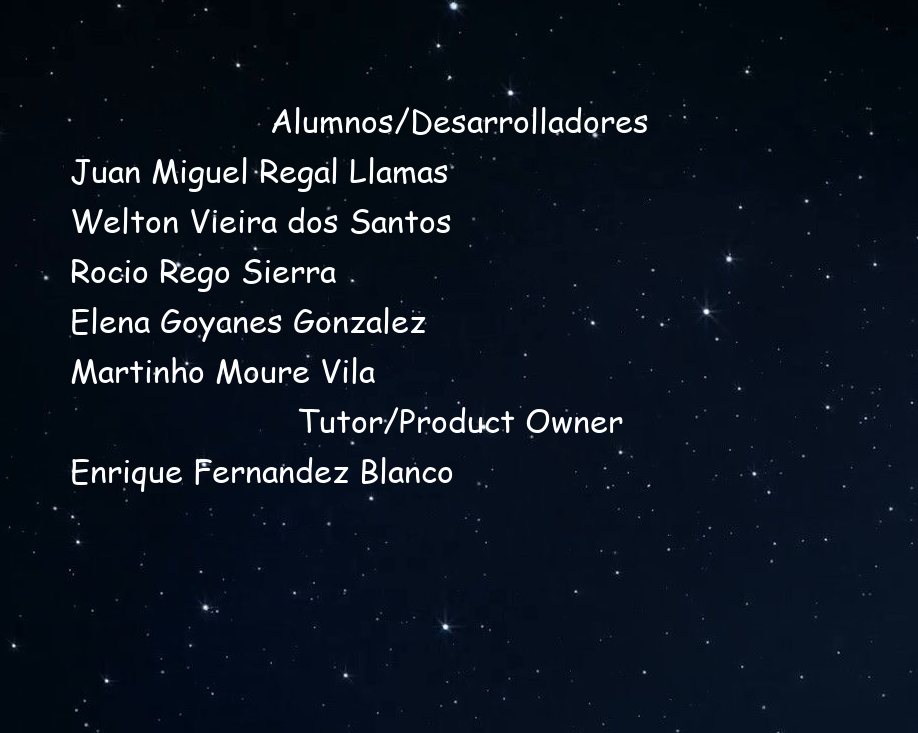
\includegraphics[scale=0.50]{imagenes/ApartadoCreditos.png}
	\caption{\label{fig:EjemploCreditos}Ejemplo del apartado créditos del menú principal}
\end{figure}

\subsubsection{Victoria}
En esta pantalla se muestra un aviso de que el jugador ha conseguido ganar y terminar el juego. Para volver al menú principal se puede pulsar la tecla Esc. Ejemplo en la Figura \ref{fig:EjemploVictoria}.

\begin{figure}[H]
	\centering
	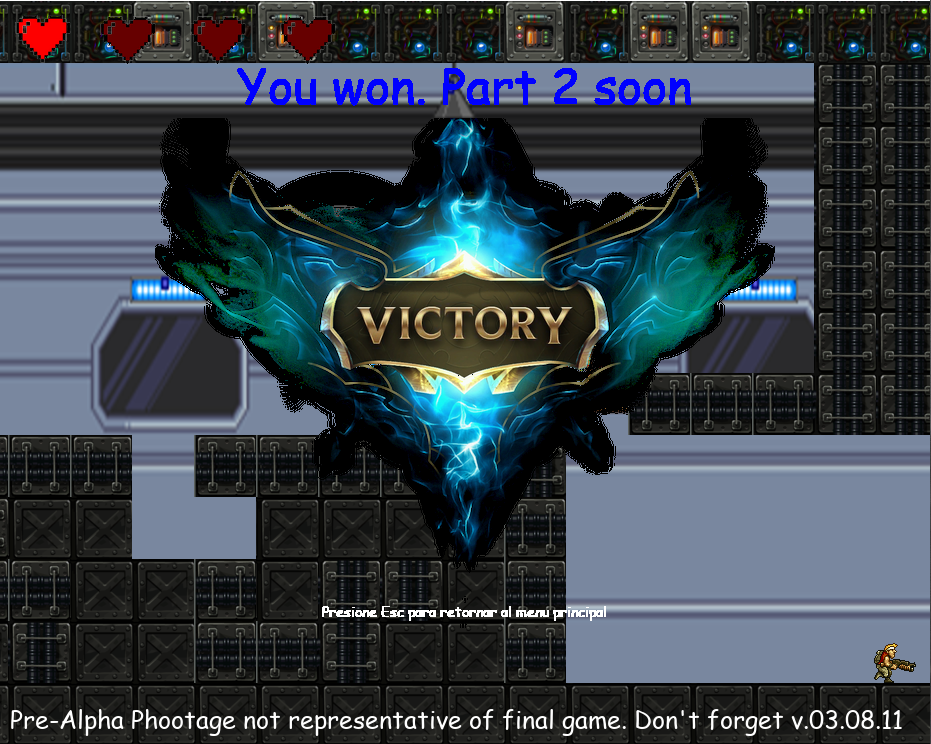
\includegraphics[scale=0.50]{imagenes/victoria.png}
	\caption{\label{fig:EjemploVictoria}Ejemplo de la escena de victoria}
\end{figure}

\subsubsection{Derrota}
Aquí se informa al jugador de que ha sido derrotado, tras haberse quedado sin vidas. Desde esta pantalla se puede volver al menú principal pulsando a tecla Esc. Ejemplo en la Figura \ref{fig:EjemploDerrota}.

\begin{figure}[H]
	\centering
	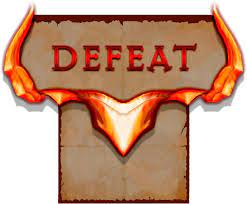
\includegraphics[scale=0.60]{imagenes/derrota.png}
	\caption{\label{fig:EjemploDerrota}Ejemplo de la escena de derrota}
\end{figure}

\subsubsection{Pausa}
Aquí se informa al jugador de que el juego sido pausado despues de precionar la tecla de escape (esc). Desde esta pantalla se puede volver al menú principal pulsando a tecla Esc o seleccionar la opción \textbf{Menu Principal}. Ejemplo en la Figura \ref{fig:EjemploPausa}.

\begin{figure}[H]
	\centering
	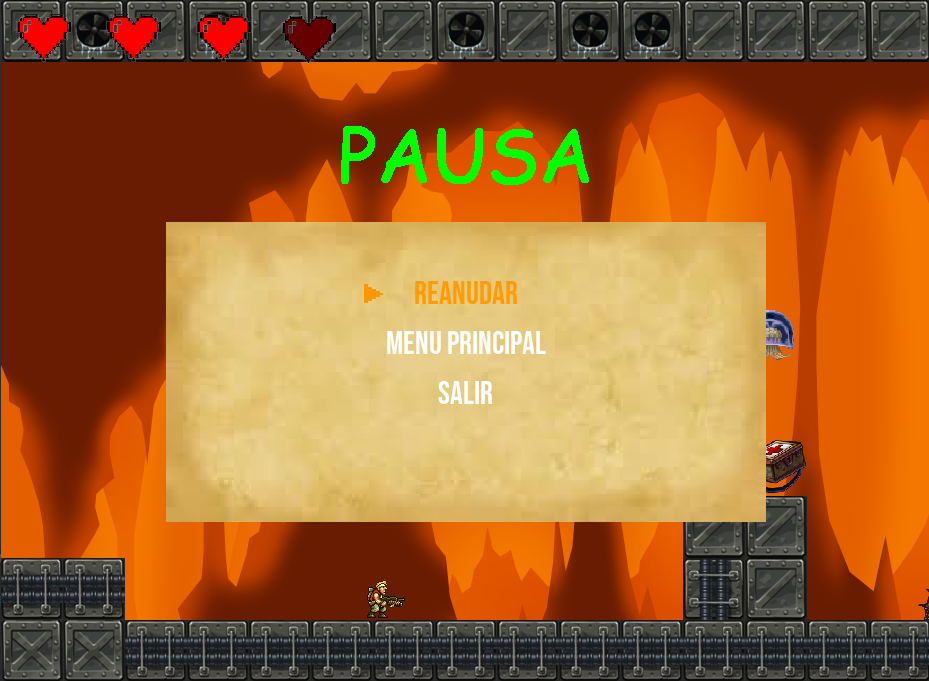
\includegraphics[scale=0.50]{imagenes/Pausa.png}
	\caption{\label{fig:EjemploPausa}Ejemplo de pausar el juego}
\end{figure}

\subsection{Aspectos destacables y detalles de su implementación}

\subsubsection{Creacción de las fases}
Un aspecto del proyecto que cabe destacar es la forma en que se crean los escenarios y se posicionan los enemigos e items, esta parte se realiza a través de una arquitectura dirigida por datos, donde cada escenario está representado por una matriz de números en un fichero .txt, donde cada número representa un tipo de bloque diferente y los ceros que no hay ningún bloque. 

Los tipos de bloque (“tiles”) están representados en ficheros json, con un array de elementos, cada uno con un identificador que corresponde al valor numérico en la matriz. El nombre de la hoja de sprites que contiene el sprite del bloque y la posición en la hoja de sprites. 

La colocación de los enemigos y los items es parecida:  

Para cada enemigo y para cada item tenemos un fichero json formado por un array de elementos. Estos elementos contienen un nº identificador, la posición en el eje x y la posición en el eje y. 

Después estos datos son leídos por las funciones: 

“readMatrix” : Para leer a matriz que representa o escenario 

“readPosition”: Para leer de las posiciones de los items y los enemigos 

“ReadTileReferences”: para leer o json que define los bloques (“tiles”) 

\subsubsection{Dinámicas de ataques}

Tanto para los disparos del personaje, como para los enemigos y los items, para que no se crearan y destruyeran objetos de forma que acabara pasando el recolector de basura provocando que se atasque el juego, todos estos elementos son creados al iniciarse el nivel, y al tener que ser destruidos son cambiados del grupo al que corresponden a un grupo que no se actualiza, por lo que se mantienen sus referencias de modo que el juego no se atasca borrandolos, pero tampoco se pierde tiempo de ejecución actualizándolos. 

Para los disparos, creamos un array de un nº máximo de balas suficientes para que se puedan reutilizar sin que el jugador se entere, este array pertenece al personaje que las dispara y sus balas al inicializarse pertenecerán al grupo de balas que no se actualizan, así, cada vez que dispare llamará a una función que le reinicia todos los atributos a la bala y esta se añade al grupo de balas que sí se actualizan. 

En el protagonista al disparar se calculará el ángulo de disparo del ratón respecto al protagonista. 

\section{Videojuego en 3D}

\subsection{Descripción}
ISS Manticore 3D es un First Person Shooter(FPS), donde el protagonista debe superar diferentes desafios hasta alcanzar su objetivo. Para ello dispondrá de armamento del que se podrá ayudar para derrotar a los distintos enemigos que tratarán de entorpecer su paso. Al comienzo de la aventura tendrá que desplazarse hasta encontrar las dos palancas que le permitiran pasar a la siguiente fase, durante este trayecto irá eliminando a los enemigos que se crucen en su camino. Una vez completado este desafío, el personaje tendrá que arreglar un motor, para ello ha de permanecer en la zona en que se encuentra el motor durante un tiempo suficiente, esto no va a resultarle tarea fácil puesto que habrá multiples enemigos tratando de dañarlo. Finalmente tendrá que conseguir llegar a una pequeña nave de emergencia, ayudandose de las plataformas que se encontrará por el espacio y le permitirán alcanzar la nave. 

\subsection{Personajes}

En esta entrega 3D, solamente tendrá un personaje principal, es decir, el mismo aventurero y cariñoso Jackie.

Como en la entrega 2D, el protagonista tendrá que completar distintas fases, en las que tendrá que superar distintos enemigos y acometer distintas tareas para alcanzar su objetivo, para ello el jugador tendrá que mover al protagonista empleando las flechas del teclado para avanzar, esquivar a los enemigos y recoger los coleccionables necesarios y disparando con un click de ratón a los distintos personajes que se interpongan en su camino. La dinámica es la misma a excepción de que ahora se pondrá acompañar el personaje en primera persona y que el manejo de la visión de Jackie se efectuará desde el ratón.

\subsection{Enemigos}

\begin{itemize}
	\item \textbf{Bot Enemy:} Enemigo a distancia que dispara y causa daño
	\begin{figure}[H]
		\centering
		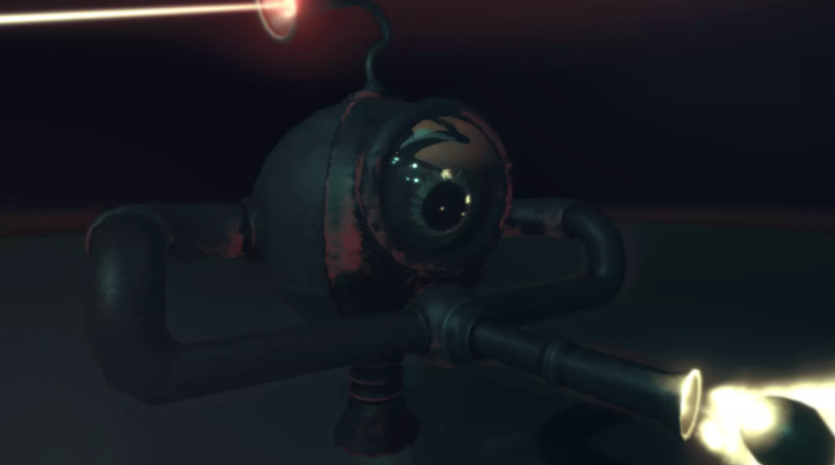
\includegraphics[scale=0.60]{imagenes/BotEnemy.png}
		\caption{\label{fig:BotEnemy}Ejemplo del Bot Enemy}
	\end{figure}
	\item \textbf{Spider Bot Enemy:} Enemigo a melee \footnote{Melee: expresión para indicar que hay una lucha cuerpo a cuerpo}.

	\begin{figure}[H]
		\centering
		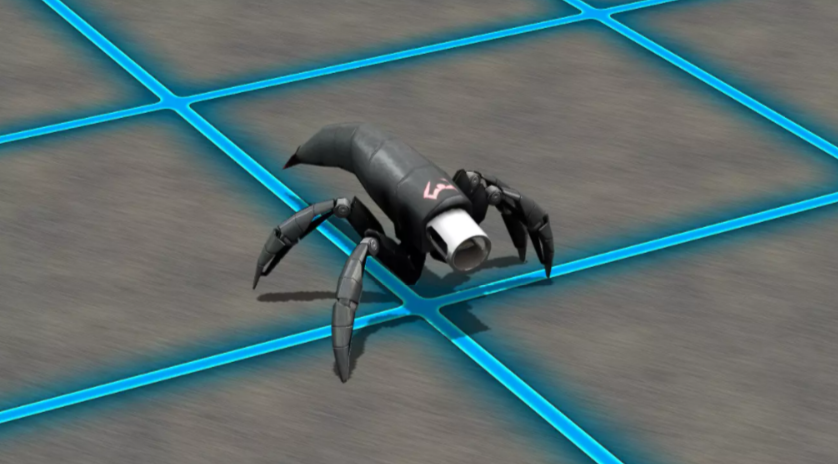
\includegraphics[scale=0.60]{imagenes/SpiderBotEnemy.png}
		\caption{\label{fig:SpiderBotEnemy}Ejemplo del Spider Bot Enemy}
	\end{figure}
\end{itemize}



\subsection{Diseño}

\subsubsection{Diseño del HUD - Patrón Observador}
El HUD consta de varios elementos:
\begin{itemize}
	\item \textbf{Tiempo:} Indica cuanto tiempo se lleva en el nivel.
	\item \textbf{Puntos:} Indica la puntuación del jugador matando enemigos.
	\item \textbf{Vidas:} Indica cuanta vida le queda al jugador.
	\item \textbf{Objetivo:} Explica al jugador cual es su objetivo actual, diciéndole a donde tiene que ir o qué tiene que hacer.
	\item \textbf{Munición:} Indica cuanta munición le queda al arma del jugador.
	\item \textbf{\% Reparación:} Exclusivo del 2º nivel, indica el porcentaje de la reparación del motor llevada a cabo.
\end{itemize}

En la Figura \ref{fig:PantallaHUD3D} muestra un ejemplo de visualización del HUD en pantalla.

\begin{figure}[H]
	\centering
	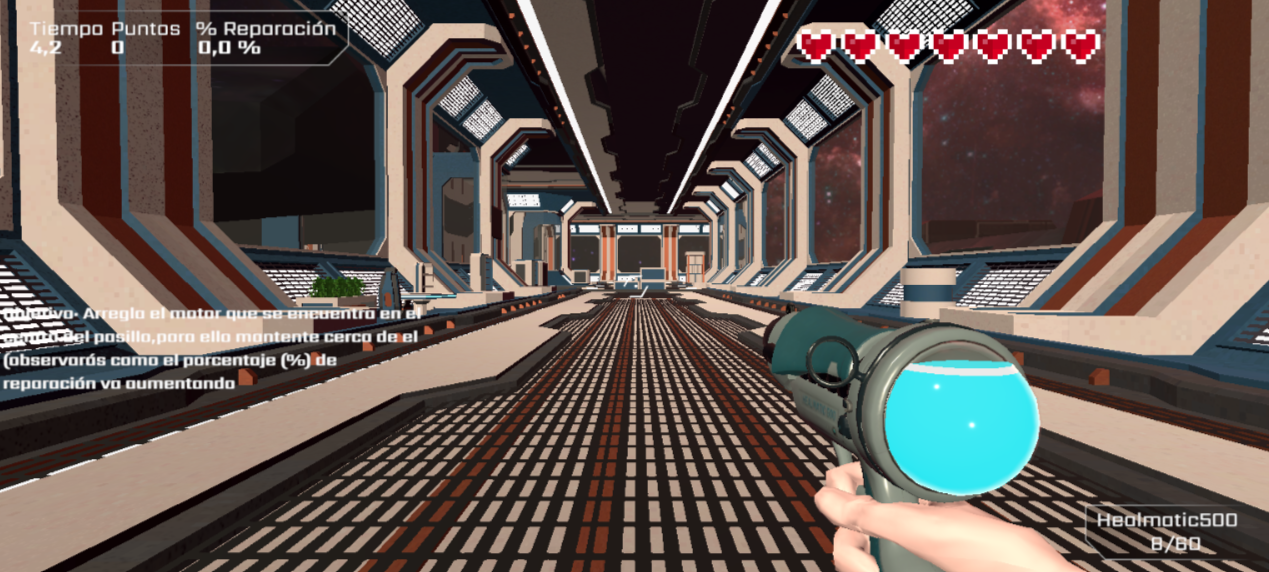
\includegraphics[scale=0.45]{imagenes/PantallaHUD3D.png}
	\caption{\label{fig:PantallaHUD3D}Ejemplo de la visualización del HUD en pantalla}
\end{figure}

El menú de pausa consta de estos elementos:
\begin{itemize}
	\item \textbf{Continuar:} Para quitar el menú de pausa y seguir con el juego
	\item \textbf{Menu principal:} Para volver al menú principal.
	\item \textbf{Salir:} Para salir del juego.
\end{itemize}
El menú de derrota, que aparece cuando el jugador pierde toda su vida consta de estos elementos:
\begin{itemize}
	\item \textbf{Reiniciar nivel:} Para reiniciar el nivel actual.
	\item \textbf{Menu principal:} Para volver al menú principal.
	\item \textbf{Salir:} Para salir del juego.
\end{itemize}

\subsubsection{Diseño de las escenas}
La 1º escena utiliza como base de la escena el prefab de una de las naves disponibles en el paquete "Federation Corvette F3", donde el jugador se moverá por su superficie, aparte se han añadido varios obstáculos y paredes en el escenario. Se han repartido enemigos por el escenario para dificultar el avance del jugador, también se han añadido dos palancas, una en el extremo de la nave, con una luz potente para que se fácil saber hacia donde dirigirse, y la 2º en una plataforma en el medio del escenario junto a la puerta que abren estas dos en conjunto.

En la 2º escena, que se desarrolla en el interior de la nave, el escenario está compuesto por unos pasillos en los que se encuentra el motor de la nave en el centro. En uno de los pasillos con los que intersecciona hay una puerta medio subida por donde acceden enemigos para perseguir al jugador, pero este no puede pasar por ese hueco. Al otro lado de la misma se spawnean los enemigos sin que el jugador lo vea. En uno de los extremos del pasillo, para fomentar la exploración, que el jugador se mueva por el escenario y facilitar el combate, se han colocado un spawner de un ítem de vida y un spawner de un ítem de munición.

La 3º escena, se desarrolla en el mismo lugar que el 1º nivel, pero esta vez se comienza donde el jugador entraba al 2º nivel desde el 1º, en el centro del mapa. Se han colocado plataformas estáticas y móviles que el jugador tendrá que utilizar para llegar a la pequeña nave que se encuentra posada sobre uno de las torres de la nave grande que hace de escenario. Para este nivel el script de movimiento de las plataformas que se creó también es capaz de rotarlas, pero utilizar esto en plataformas que empleará el jugador se acabó descartando porque dificultaba mucho al jugador saltar correctamente de una plataforma a otra.

\subsubsection{Zona de reparación del motor}
Para la reparación del motor, se ha creado un objeto que es un cubo invisible que se puede atravesar, el área de reparación, con un script que sigue el patrón observer, comprobando si el jugador se encuentra dentro de él o no. 

Para mostrar en la HUD el porcentaje de la reparación se han creado en el script \textit{Gamesystem.cs} las funciones ``MostrarReparacion'' (que sirve para indicar que se active el objeto del HUD que muestra el porcenaje de reparación) y ``UpdateReparacion'' (que actualiza el número que indica el porcentaje), que a su vez llaman a sus homónimos en la clase GameSystemInfo que se encuentran en el objeto GameUI, inicializado directamente por el GameSystem. 

\subsubsection{Mostrar el objetivo actual}
Para mostrar los objetivos el funcionamiento, con las funciones ``MostrarObjetivo'' y ``UpdateObjetivo'', estas funciones son llamadas al GameSystem por: 

En el 1º nivel por ``LeverSystem'', el sistema encargado del funcionamiento de las palancas, al iniciarse indicará que el objetivo es activar las palancas del escenario y dónde están localizadas. Y mediante el patrón observador, comprobará si el estado de todas las palancas es que estén activadas, entonces al haber activado todas las palancas se volverá a llamar a ``UpdateObjetivo'' para que actualice el objetivo diciéndole al jugador que tiene que atravesar el pasillo que ha abierto. 

En el 2º nivel, ``RepairZone'', el sistema encargado del funcionamiento del porcenataje de reparación, al iniciarse indicará que el objetivo es reparar el motor. Y mediante el patrón observador, comprobará si el estado del motor es que esté reparado, y entonces volverá a llamar a ``UpdateObjetivo'' para que actualice el objetivo diciendole al jugador que tiene que volver por donde vino.

En el 3º nivel, simplemente un script al iniciarse indicará que el objetivo es subir por las plataformas para llegar a una nave en la que huir, solo hay un objetivo en este nivel, por lo que no necesitará actualizarse más.

\subsubsection{Enemigos}
Respecto a los enemigos en común, comentar que utilizan el patrón plantilla siendo prefabs de Unity con varias opciones configurables. A continuación, se pueden ver los aspectos de cada uno:
\begin{itemize}
	\item \textbf{BotEnemy:} Este prefab de enemigo, parte del modelo del paquete Enemy Robots. Para este se ha creado un Script con nombre RobotAI, el cual permitirá al enemigo realizar diversas acciones. Por defecto, se moverá a través de los puntos marcados como pivots circularmente patrullando, esto permite al enemigo tener interacción propia con el sistema en el tiempo que no detecta al enemigo. Este enemigo detectará al jugador una vez este entre dentro de un rango de distancia, configurable a través del prefab, y lance un LineCast para detectar si hay algún otro objeto entre medias, así se evita que el jugador piende que el enemigo tiene una ventaja por el simple hecho de detectarlo sin llegar a verlo. Una vez detectado, el enemigo empezará a perseguir al jugador, manteniendo un mínimo de distancia con él. Consta, así mismo, de un contador entre ataques para disparar cada el tiempo indicado. Finalmente, en los ataques instancia un objeto EnemyBullet, al cual asigna un movimiento, este al colisionar con el jugador restará un punto de vida, comentar también que se ha tomado la decisión de que los disparos del enemigo sean un proyectil, y no hitscan (disparo inmediato sin tiempo de viaje), con un movimiento más lento y retardo a la hora de apuntar para darle ventaja al jugador y que no sienta que los enemigos están haciendo trampa al calcular donde atacar con precisión e inmediatez.
	\item \textbf{PA\_Warrior Variant:} Este prefab de enemigo, parte del prefab y animaciones PA\_Warrior del paquete SciFi Enemies and Vehicles. Nuevamente se ha creado un Script para dichos enemigos, estes incluyen el comportamiento inteligente dado por Unity para navegar hasta la posición del jugador. Una vez más tiene un contador para medir el tiempo entre ataques. Una vez se complete el tiempo de ese contador, si se encuentra en un rango suficientemente cercano del jugador iniciarán la animación de ataque y provocarán daño en el jugador. Se ha tomado la decisión de que los enemigos provoquen daño reducido al jugador, pero como persiguen y atacan muchos juntos son un tipo de enemigo más diverso. Mencionar, como patrón utilizado, la máquina de estados proporcionada por Unity para la animación. Vease Figura \ref{fig:MaquinaEstados}.
\end{itemize}

\begin{figure}[H]
	\centering
	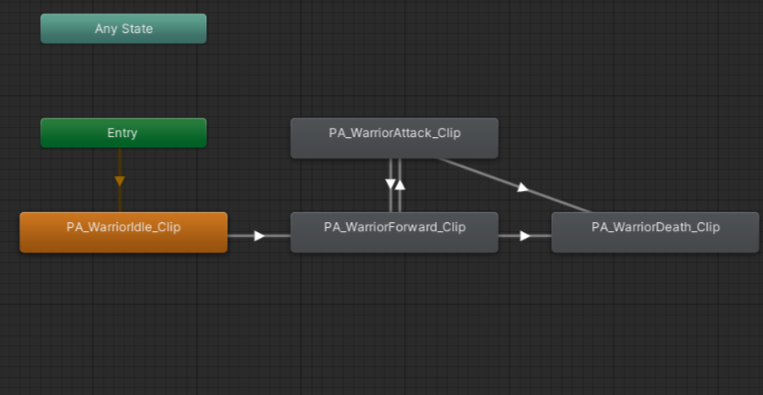
\includegraphics[scale=0.65]{imagenes/MaquinaEstados.png}
	\caption{\label{fig:MaquinaEstados}Ejemplo de la visualización del HUD en pantalla}
\end{figure}

\subsubsection{Puntuación}
Cada vez que se elimina a un enemigo se suma un punto a la puntuación del jugador, que puede observar en la parte superior izquierda del HUD. Este sistema sigue un patron comando, pues cada vez que se ejecuta este ordena al HUD que actualice la puntuación.

\subsubsection{Sistema de palancas}
En cuanto al sistema de palancas, se utiliza el prefab de la palanca y su correspondiente animación, visible cuando el personaje la acciona. Se ha modificado el script propio de la palanca para obtener Lever con el comportamiento deseado. Además, se ha creado otro script nuevo para el sistema, denominado LeverSystem, que permite que, al añadir a la escena tantas palancas como se deseen, solo se abra la puerta cuando todas y cada una de ellas estén accionadas.

\subsubsection{Sistema de vidas}
El sistema de vidas gestiona la salud del personaje, cuando una bala de un bot enemy golpea al personaje, este pierde una vida. En cambio, cuando es un spiderbot el que alcanza al personaje, este se queda sin un cuarto de vida. También permite al personaje recuperar vida cuando este recoge un ítem de vida. Cuando el personaje se queda sin vidas el sistema muestra el menú de Game Over donde el jugador puede escoger entre reiniciar el nivel en el que se encuentra, volver al menú principal o abandonar el juego.

\subsubsection{Items de recuperación de munición y vida}
Para estos items se ha utilizado utilizado unos modelos con forma de maletines, para la munición se utiliza el script ``Ammo Box'' del ``Creator Kit: FPS'', y recupera 10 unidades de munición.

En el caso del item de vida, se creó un script con un funcionamiento similar al de munición, al colisionar el jugador con el item este llama a la función de recuperar vida y se destruye.

Estos dos scripts siguen un patrón comando pues ordenan actualizar los datos de munición (Figura \ref{fig:EjemploMunicion3D}) y de vida (Figura \ref{fig:EjemploVida3D}).

\begin{figure}[H]
	\centering
	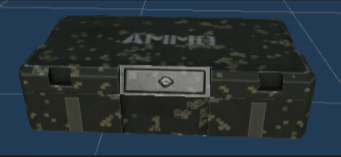
\includegraphics[scale=0.65]{imagenes/EjemploMunicion3D.png}
	\caption{\label{fig:EjemploMunicion3D}Ejemplo de un recolectable de munición}
\end{figure}

\begin{figure}[H]
	\centering
	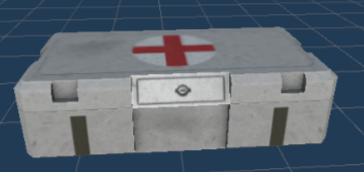
\includegraphics[scale=0.65]{imagenes/EjemploVida3D.png}
	\caption{\label{fig:EjemploVida3D}Ejemplo de un recolectable de vida}
\end{figure}

\subsubsection{Objeto de cambio de escena}
Para el cambio de escena de cada nivel se ha utilizado un prefab (por lo que sigue el patrón plantilla) que es un cubo invisible con el script ``ChangeScene'', este se activa cuando el jugador entra en contacto con el objeto cargando el escenario indicado. Al ordenar cambiar de escenario siguen un patrón comando.

\subsubsection{Menu de pausa}
Se utilizó el menu de pausa proporcionado por ``Creator Kit: FPS'' pero cambiando el botón de seleccion de nivel por un botón para ir menú principal.

\subsubsection{Jugador, controlador del jugador y sistema de disparos}
Para estos 3 elementos se utilizaron los proporcionados por "Creator Kit: FPS" y no se realizó ningún cambio destacable en ellos.

\subsection{Escenas}

La transición entre escenas se muestra en el diagrama de la Figura \ref{fig:TrasicionEscenas3D}. 

\begin{figure}[H]
	\centering
	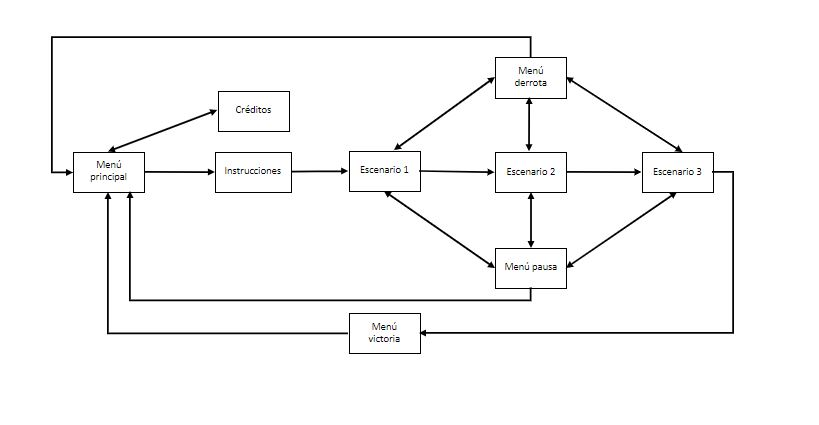
\includegraphics[scale=0.60]{imagenes/transicionEscenas3D.png}
	\caption{\label{fig:TrasicionEscenas3D}Diagrama de transición de las escenas}
\end{figure}

\subsubsection{Menú principal}
El menú principal consta de 3 botones como se muestra en la Figura \ref{fig:MenuPrincipal3D1}.
\begin{figure}[H]
	\centering
	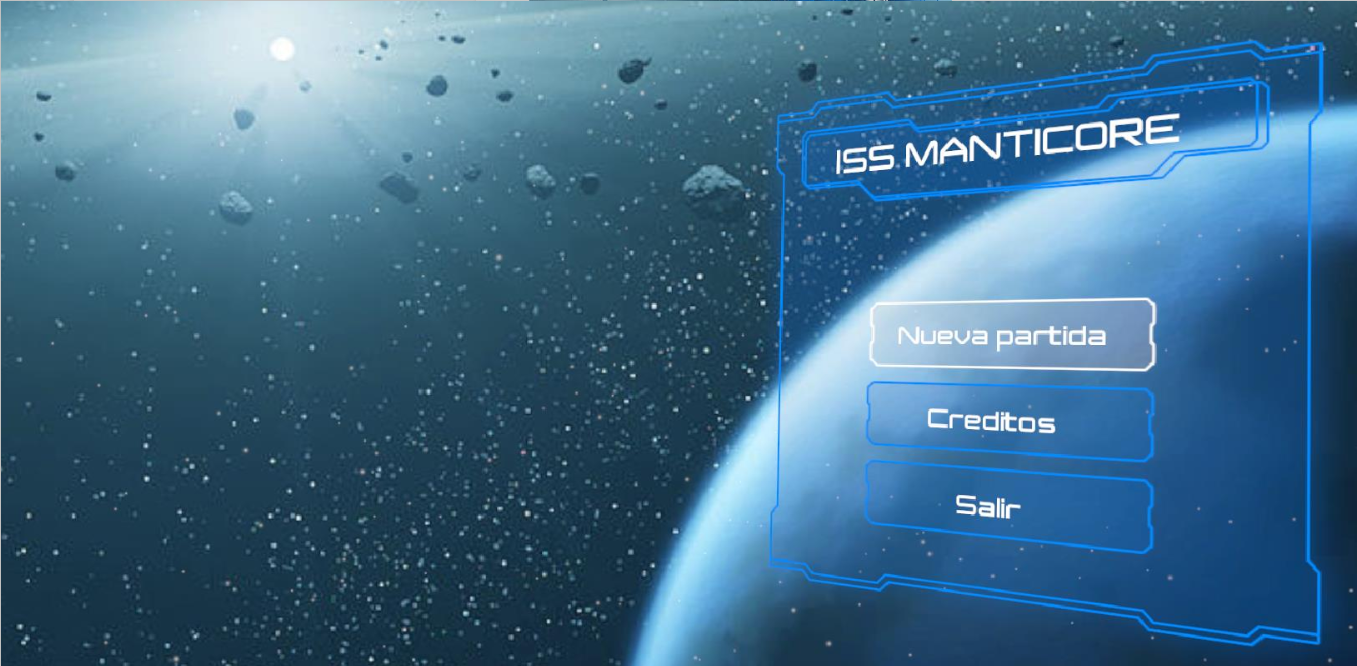
\includegraphics[scale=0.35]{imagenes/MenuPrincipal3D1.png}
	\caption{\label{fig:MenuPrincipal3D1}Ejemplo del Menu Principal}
\end{figure}

Detalles de cada opción del menu presentado en la Figura \ref{fig:MenuPrincipal3D1}:
\begin{itemize}
	\item \textbf{Nueva Partida:} Activa una segunda ventana en el menú con una explicación de los controles del juego y un botón ``Continuar al juego'' que lleva al nivel 1 como se muestra en la Figura \ref{fig:MenuPrincipalNuevaPartida}.
	\begin{figure}[H]
		\centering
		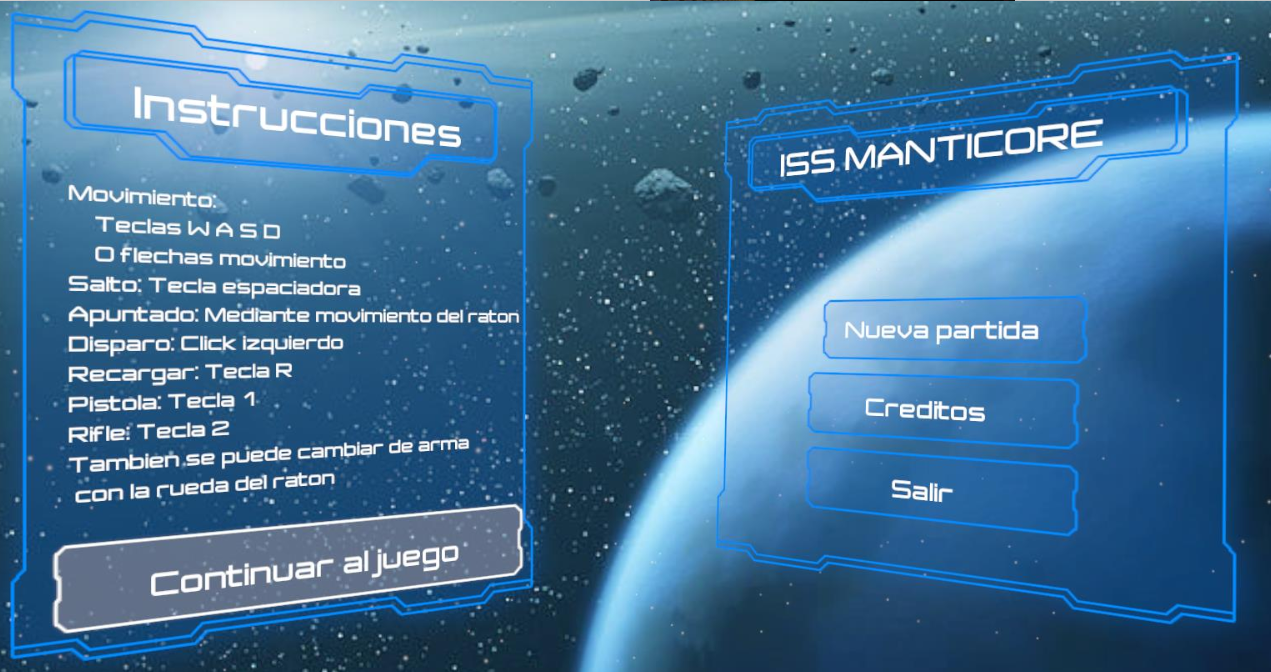
\includegraphics[scale=0.40]{imagenes/MenuPrincipalNuevaPartida.png}
		\caption{\label{fig:MenuPrincipalNuevaPartida}Apartado Nueva partida del Menu Principal}
	\end{figure}
	\item \textbf{Créditos:} Activa una segunda ventana en el menú con los créditos del juego y un botón ``cerrar'' para cerrar esta ventana como se muestra en la Figura \ref{fig:MenuPrincipalCreditos}.
	\begin{figure}[H]
		\centering
		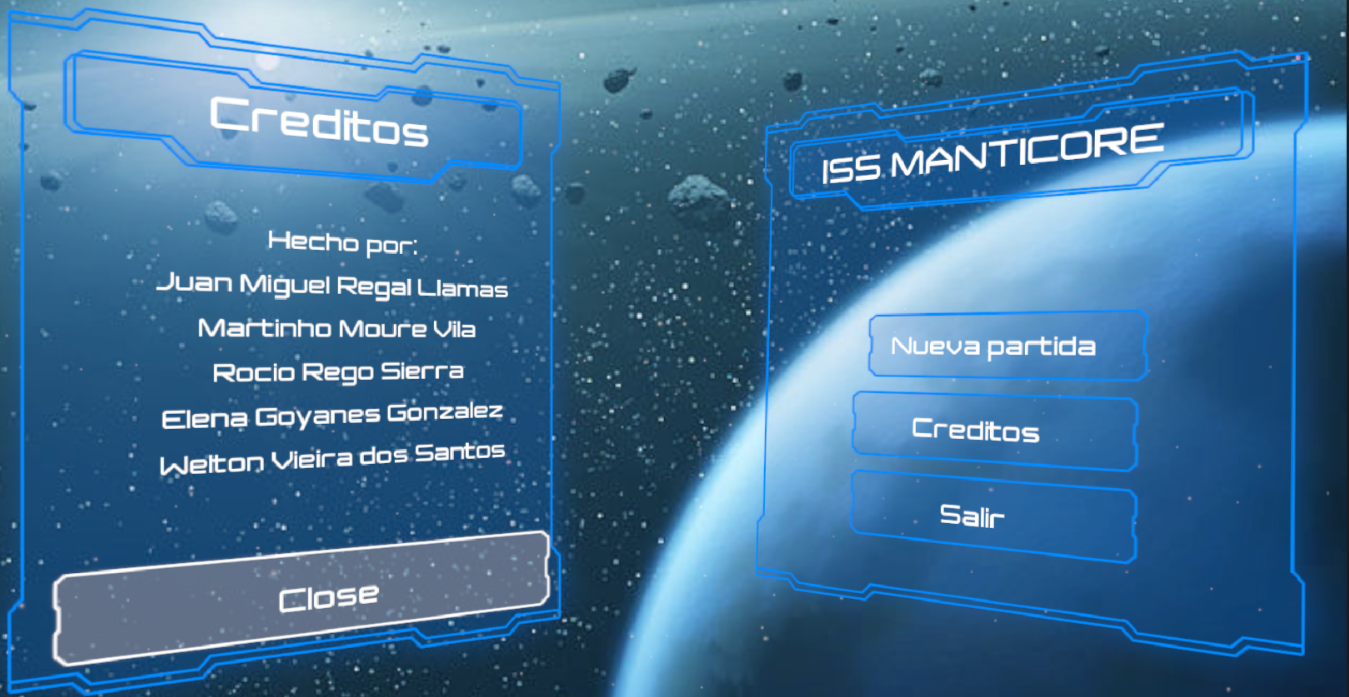
\includegraphics[scale=0.35]{imagenes/MenuPrincipalCreditos.png}
		\caption{\label{fig:MenuPrincipalCreditos}Apartado Crédito del Menu Principal}
	\end{figure}
	\item \textbf{Salir:} Cierra el juego.
\end{itemize}


\subsubsection{Menú de derrota}
El menú de derrota consta de un texto informativo para indicar que se ha terminado el juego con una frase ``Game Over'' y tres opciones al usuario (Figura \ref{fig:MenuDerrota}):
\begin{itemize}
	\item \textbf{Reiniciar Nivel:} Devuelve al jugador al inicio del nivel del cual ha sido derrotado.
	\item \textbf{Menu Principal:} Devuelve al jugador al Menu Principal del juego.
	\item \textbf{Salir}: Permite el jugador salir del juego.
\end{itemize}

\begin{figure}[H]
	\centering
	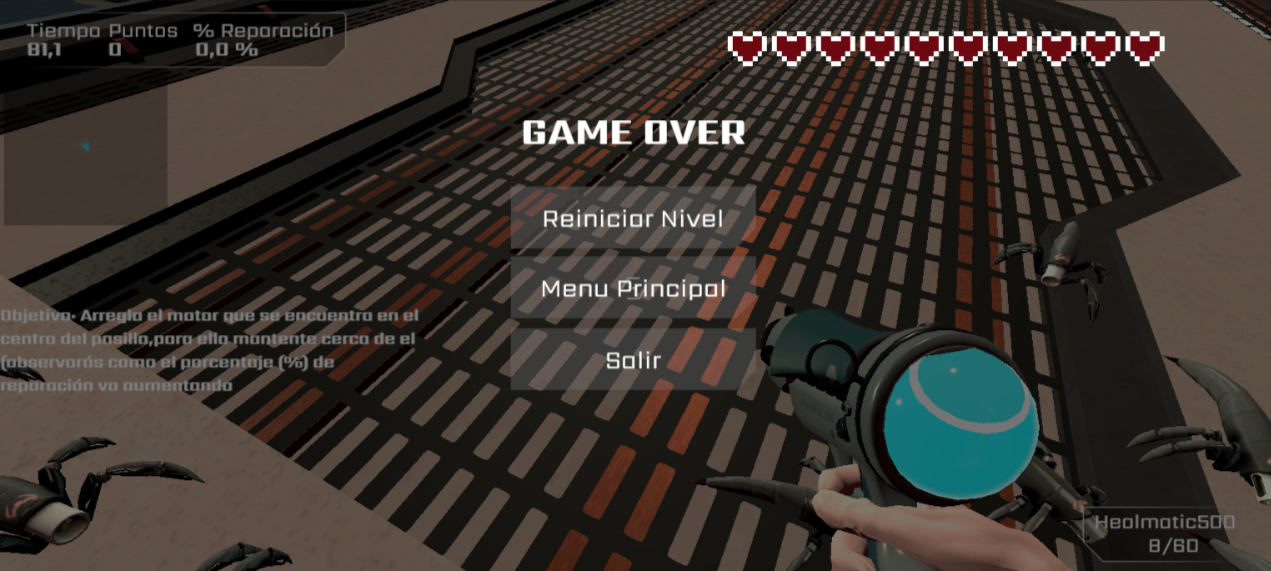
\includegraphics[scale=0.40]{imagenes/MenuDerrota.png}
	\caption{\label{fig:MenuDerrota}Ejemplo de la pantalla de derrota}
\end{figure}

\subsubsection{Menú de victoria}
El menú de victoria consta de un texto informativo para indicar que se ha completado el juego (Figura \ref{fig:MenuVictoria3D}), y consta de 1 botón:
\begin{itemize}
	\item \textbf{Reiniciar Juego:} Devuelve al jugador al Menú Principal (Figura \ref{fig:MenuPrincipal3D1}), donde podrá escoger que acción tomar.
\end{itemize}

\begin{figure}[H]
	\centering
	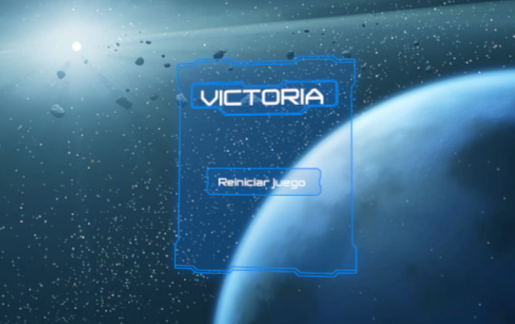
\includegraphics[scale=0.85]{imagenes/MenuVictoria3D.png}
	\caption{\label{fig:MenuVictoria3D}Ejemplo de la pantalla de victoria}
\end{figure}

\subsubsection{Menú de pausa}
El menú de pausa consta de tres botones para que el jugador pueda elegir una de las opciones (Figura \ref{fig:MenuPausa}):
\begin{itemize}
	\item \textbf{Continuar:} Permite que el jugador pueda continuar la partida.
	\item \textbf{Menu Principal:} Permite que el jugador pueda regresar al Menu Principal del juego.
	\item \textbf{Menu Salir:} Permite que el jugador pueda salir del juego.
\end{itemize}


\begin{figure}[H]
	\centering
	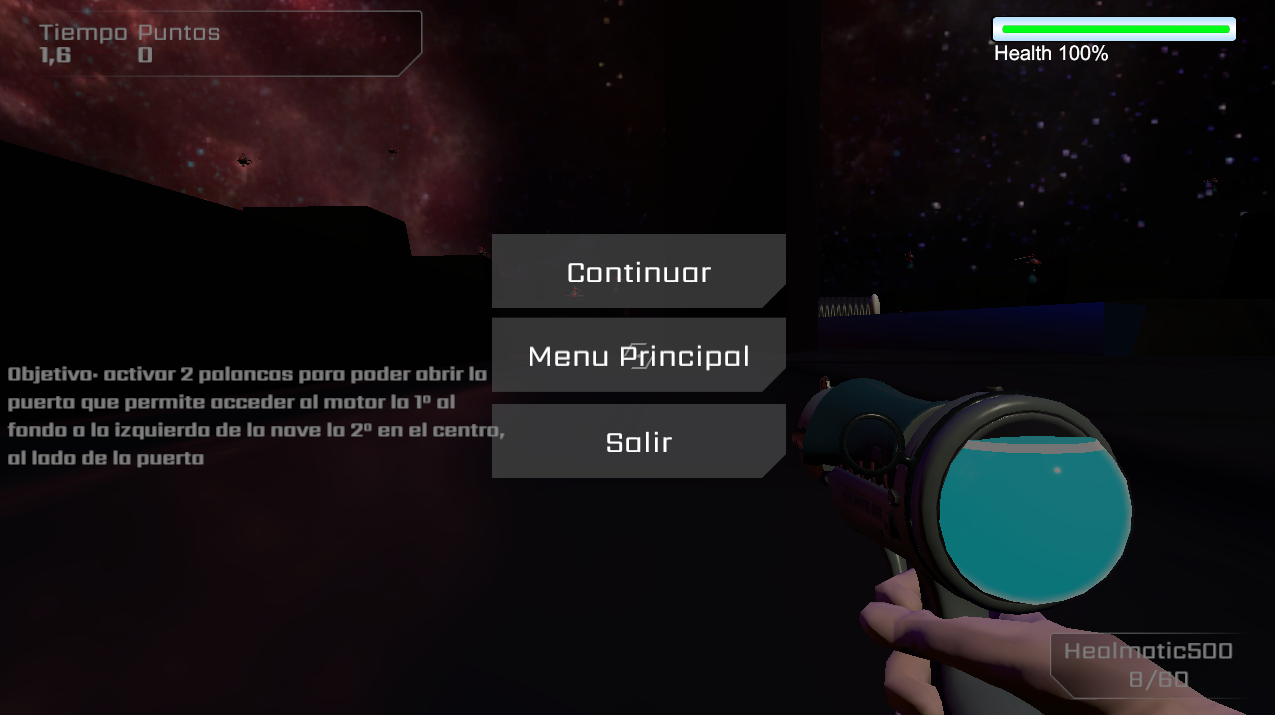
\includegraphics[scale=0.85]{imagenes/MenuPausa.png}
	\caption{\label{fig:MenuPausa}Ejemplo de la pantalla de pausa}
\end{figure}

\subsubsection{Escena 1}
La primera fase empieza en un extremo del escenario, el personaje debe recorrerlo hasta encontrar las dos palancas (Figura \ref{fig:Palanca}) que debe accionar para conseguir pasar al siguiente nivel, durante el trayecto por el escenario el personaje ha de eliminar a los enemigos que intentarán dificultar su devenir.

\begin{figure}[H]
	\centering
	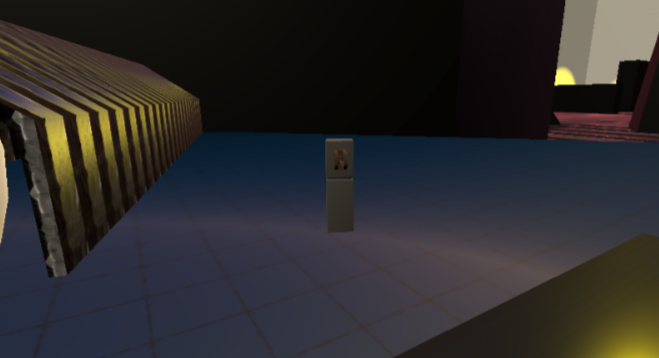
\includegraphics[scale=0.75]{imagenes/Palanca.png}
	\caption{\label{fig:Palanca}Ejemplo de la palanca}
\end{figure}

La única forma de superar esa fase es accionando dos palancas, que se encuentran distribuidas por el escenario y permiten abrir la puerta que da acceso al siguiente nivel.

Para el diseño de este escenario se han utilizado los Prefabs que proporcionan los siguientes paquetes:
\begin{itemize}
	\item \textbf {Creator kit - FPS:} Se utiliza como base para el personaje,su controlador, el sistema de disparos, el menú de pausa y el HUD
	\item \textbf{SpaceSkies Free:} Se utiliza uno de sus assets como skybox
	\item \textbf{Federation Corvette F3:} Se utiliza como base del escenario
	\item \textbf{Interactive Physical Door Pack:} Se utiliza como base para crear las palancas
	\item \textbf{Simple Heart Health System:} Se utiliza como base para crear el sistema de vidas
	\item \textbf{Enemy Robots:} Se utilizan para los modelos de los enemigos
\end{itemize}


\subsubsection{Escena 2}
Para completar esta fase, será necesario arreglar un generador (Figura \ref{fig:Generador}) que se encuentra en el centro del escenario, en el cual aparecerán constantemente enemigos desde una zona no acesible que dificultarán al personaje arreglar el problema en el generador. Para realizar esta tarea se ha optado por la mecánica de capturar el objetivo lo cual sucede de forma pasiva mientras el jugador se mantenga en el área cercana. Para facilitar dicha tarea, en un pasillo externo el jugador podrá encontrar cajas de munición y vida para recuperarse y poder continuar luchando, dichos objetos apareceran cada 40 segundos. Una vez se complete, el personaje tendrá que volver por el mismo camino por el cual llegó para pasar a la última fase.

\begin{figure}[H]
	\centering
	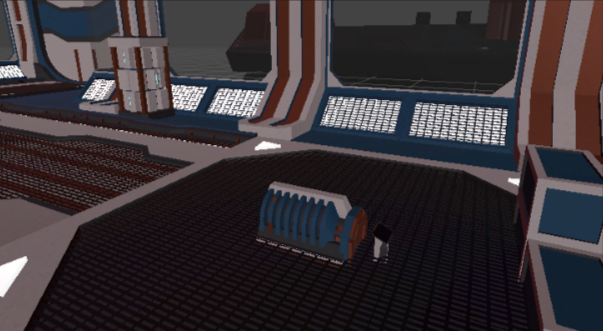
\includegraphics[scale=0.75]{imagenes/Generador.png}
	\caption{\label{fig:Generador}Ejemplo del generador}
\end{figure}

Para el diseño de este escenario se han utilizado los Prefabs que proporcionan los siguientes paquetes:
\begin{itemize}
	\item \textbf{Creator kit - FPS:} Se utiliza como base para el personaje,su controlador, el sistema de disparos, el menú de pausa y el HUD
	\item \textbf{SpaceSkies Free:} Se utiliza uno de sus assets como skybox
	\item \textbf{Federation Corvette F3:} Se utiliza como base del escenario
	\item \textbf{Simple Heart Health System:} Se utiliza como base para crear el sistema de vidas
	\item \textbf{Sci-Fi Styled Modular Pack:} Se utiliza como base para la construcción del escenario encima de la nave, con el generador y los pasillos
	\item \textbf{SciFi Enemies and Vehicles:} Se utiliza para el modelo del enemigo con sus animaciones de ataque y persecución
	\item \textbf{Boxes pack:} Se utiliza para las cajas de munición y vida
\end{itemize}


\subsubsection{Escena 3}
En esta fase el objetivo es huir de esa nave para llegar a otra pequeña nave de emergencia que se encuentra localizada en una de las torres de ese escenario. El único inconveniente que el personaje va encontrar es que él mismo tiene que buscar una forma de acceder a dicha nave de emergencia, que está localizada en un plano distinto al del protagonista.

El personaje encontrará cajas flotantes que él mismo podrá utilizar saltando sobre ellas. Una vez llegado al objetivo, el personaje entrará en dicha nave de emergencia, esa fase se dará por concluida y se dará paso a la escena del menú de victoria.

Para el diseño de este escenario se han utilizado los Prefabs que proporcionan los siguientes paquetes:
\begin{itemize}
	\item \textbf{Creator kit - FPS:} Se utiliza como base para el personaje,su controlador, el sistema de disparos, el menú de pausa y el HUD
	\item \textbf{SpaceSkies Free:} Se utiliza uno de sus assets como skybox
	\item \textbf{Federation Corvette F3:} Se utiliza como base del escenario
	\item \textbf{Sci-Fi Styled Modular Pack:} Se utiliza para los modelos de las plataformas móviles
	\item \textbf{Simple Heart Health System:} Se utiliza como base para crear el sistema de vidas
	\item \textbf{Destructor Spaceship:} Se utiliza para el modelo de nave a la que tiene que llegar el personaje
\end{itemize}

\subsection{Aspectos destacables y detalles de su implementación}

\subsubsection{Plataformas móviles}
Para la creación de plataformas móviles se ha creado un prefab que permite a través del inspector controlar el movimiento y/o rotación de la plataforma a la que este asignada. Para ambas características se permite indicar las velocidades. En lo que respecta al movimiento este se basa en una serie de puntos a través de los cuales se irá moviendo y se pueden configurar a través del inspector. Implementan el patrón plantilla al ser prefab.

Además, cabe destacar que se hace uso de la herramienta ProBuilder de Unity para crear varios objetos de las escenas 1 y 3, empleando los prefabs disponibles, y también para crear un objeto con paredes invisibles que sirve para delimitar los escenarios.
